\begin{figure*}[!t]
\begin{tabular}{ccc}
\begin{minipage}[t]{0.23\hsize}
    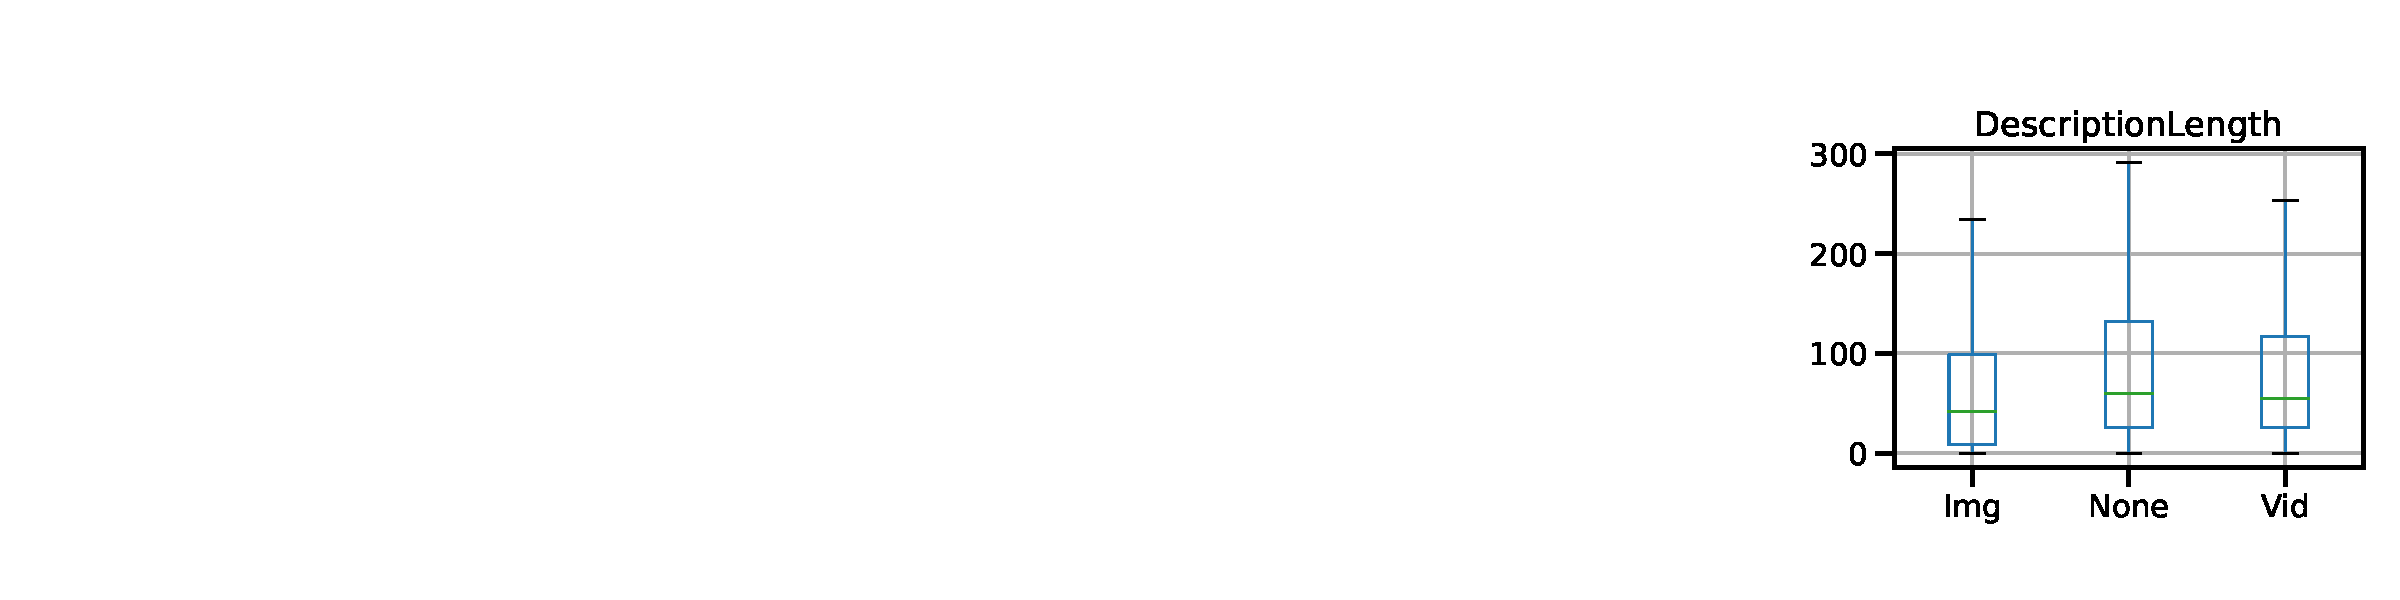
\includegraphics[width=1\linewidth]{./figures/words.pdf}
    \caption{Distribution of \#~words (``Report'' dimension)}
    \label{fig:words}
\end{minipage}
\hspace{0.04\columnwidth}
\begin{minipage}[t]{0.46\hsize}
    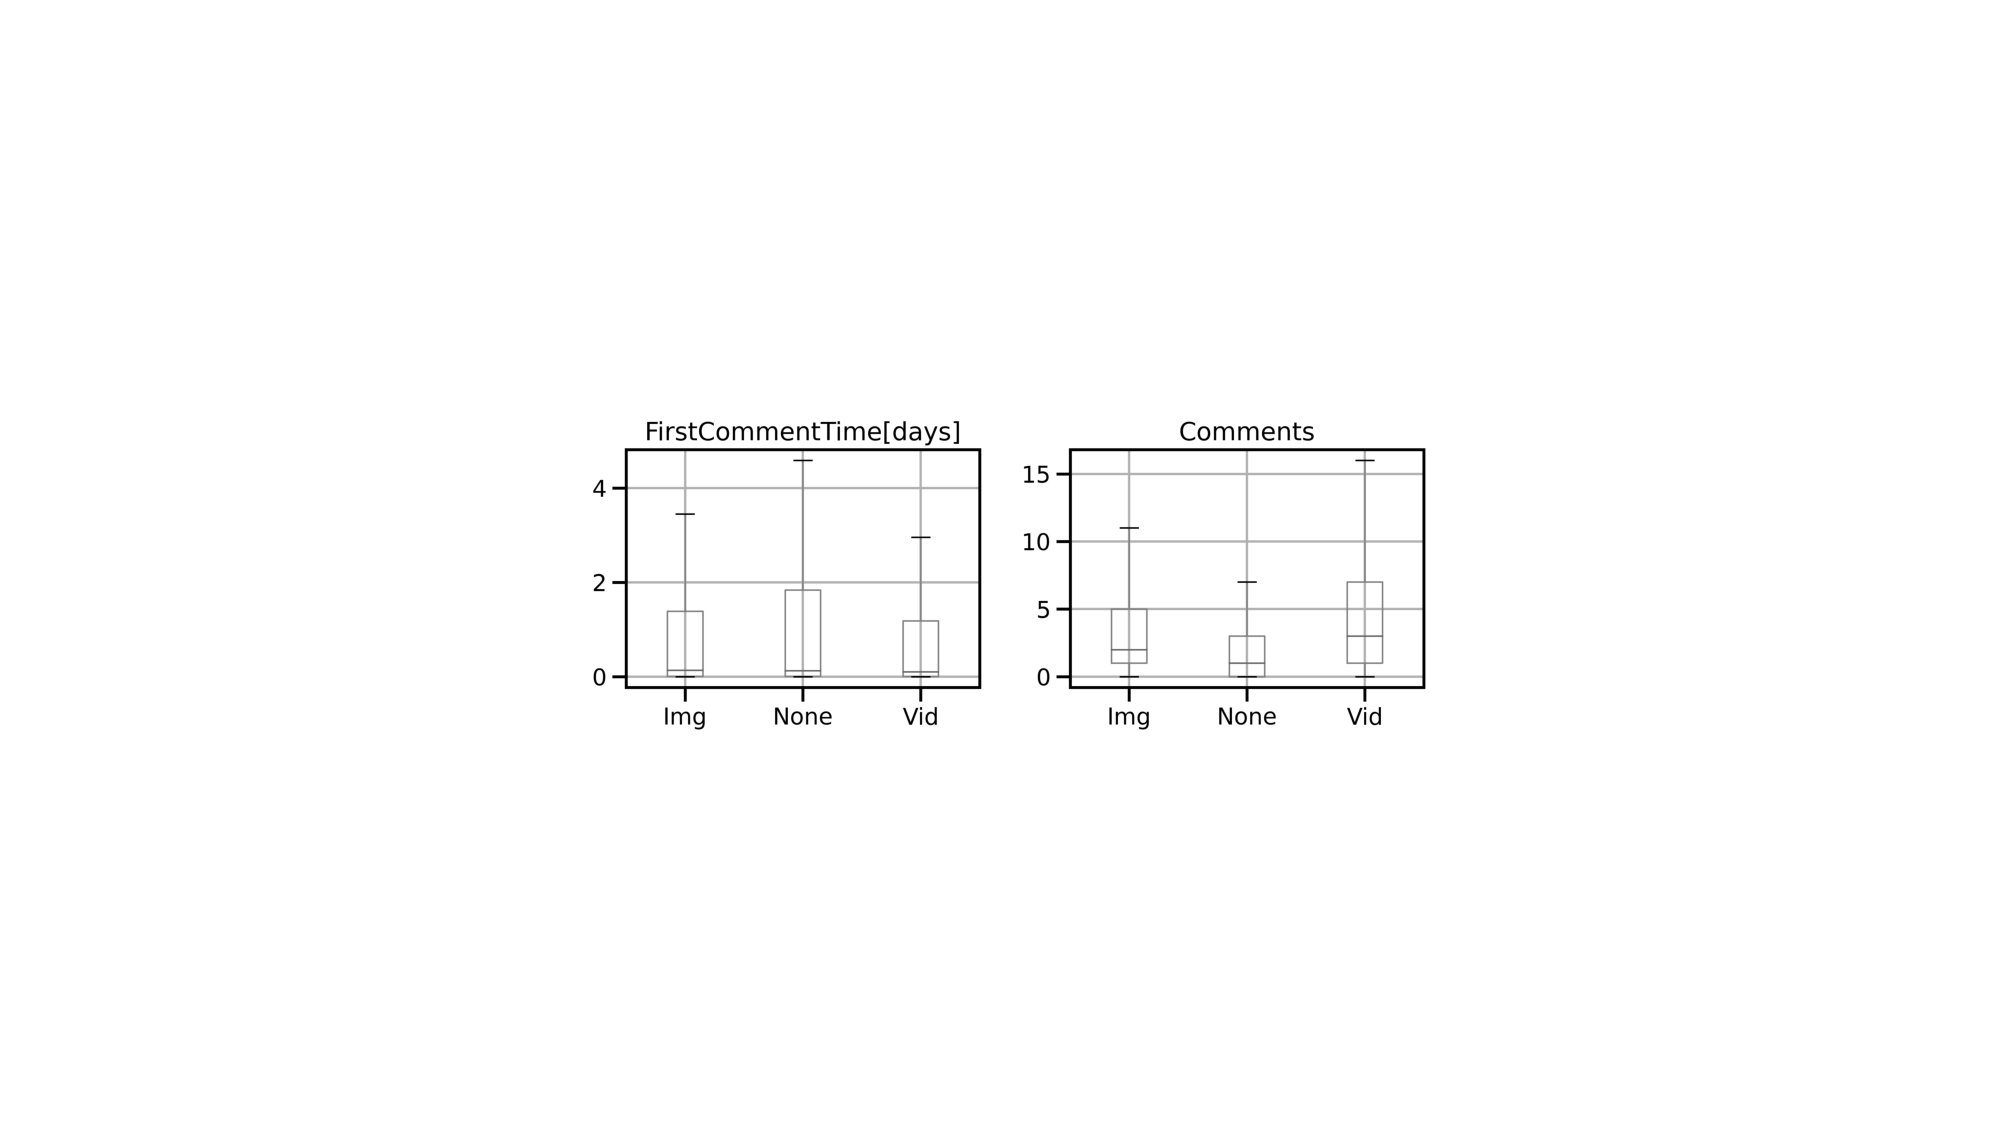
\includegraphics[width=1\linewidth]{./figures/discussions.pdf}
    %\caption{Amount of texts written in issue reports. }
    % \caption{The attributes in the Discussion dimension}
    \caption{Distribution of days to receive the first comments and the number of comments (``Discussion'' dimension)}
    \label{fig:discussion}
\end{minipage}
\hspace{0.04\columnwidth}
\begin{minipage}[t]{0.23\hsize}
    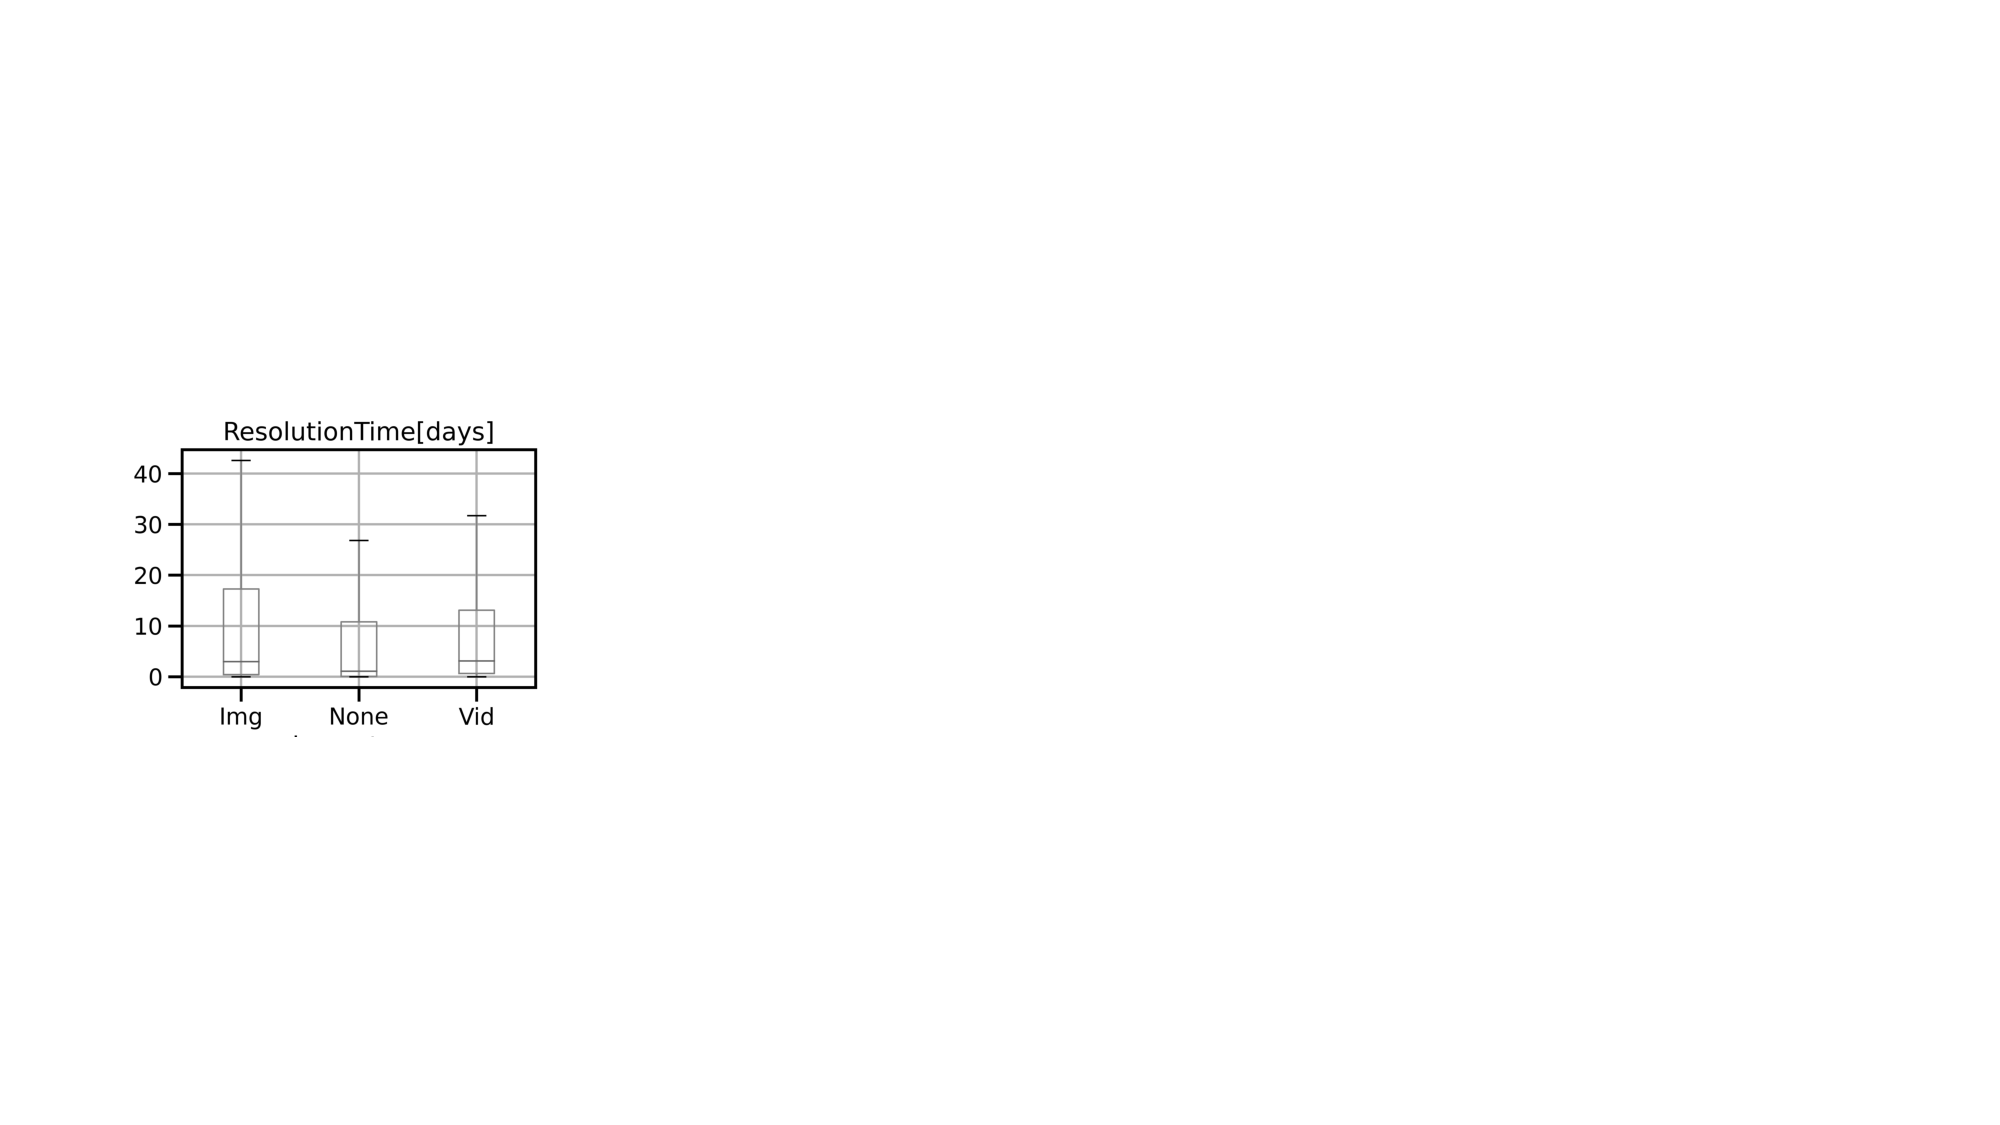
\includegraphics[width=1\linewidth]{./figures/fixes.pdf}
    \caption{Distribution of resolution time (``Fix'' dimension)}
    \label{fig:resolvedtime}
\end{minipage}
\end{tabular}
\end{figure*}



\section{Results}
\label{sec:results}

% 初期段階の調査として,画像及び動画がissueの各attributesに
% 与える影響について調査する.
% 表2で得られたそれぞれのカテゴリ間で比較を比較を行う.
% 等分散性を仮定できないデータが含まれていたため,
% 比較にはSteel-Dwass testを採用する.
% 
% visualizationは,issueの解決時間,
% コメント数,文字数に何らかの影響を与える.
% 検定結果を表6に示す.
% 有意水準は0.05を採用する.
% IssueResolvedTimeにおいて,
% ImgとMovは片側検定で有意差があった.
% また,表Xより,平均値,中央値でNoneカテゴリの
% issueよりImgとMovカテゴリのissueの方が
% 課題解決時間が長かった.
% よって,画像もしくは動画がissue作成時に付与
% される課題はその解決時間が有意に長くなる.
% また,#comments及び#charsでは両側検定で
% 有意であり,これらのattributesにも
% 有意な影響を与えることがわかった.
% ただし,imageとvideos に有意差は
% 観測されなかった.

% As an initial analysis, we investigated 
% the impact of images and videos on 
% the issues in terms of the attributes. 
% As an initial analysis, 


\subsection*{RQ1: \RQone{}}
% \begin{figure}[t]
%     \centering
%     %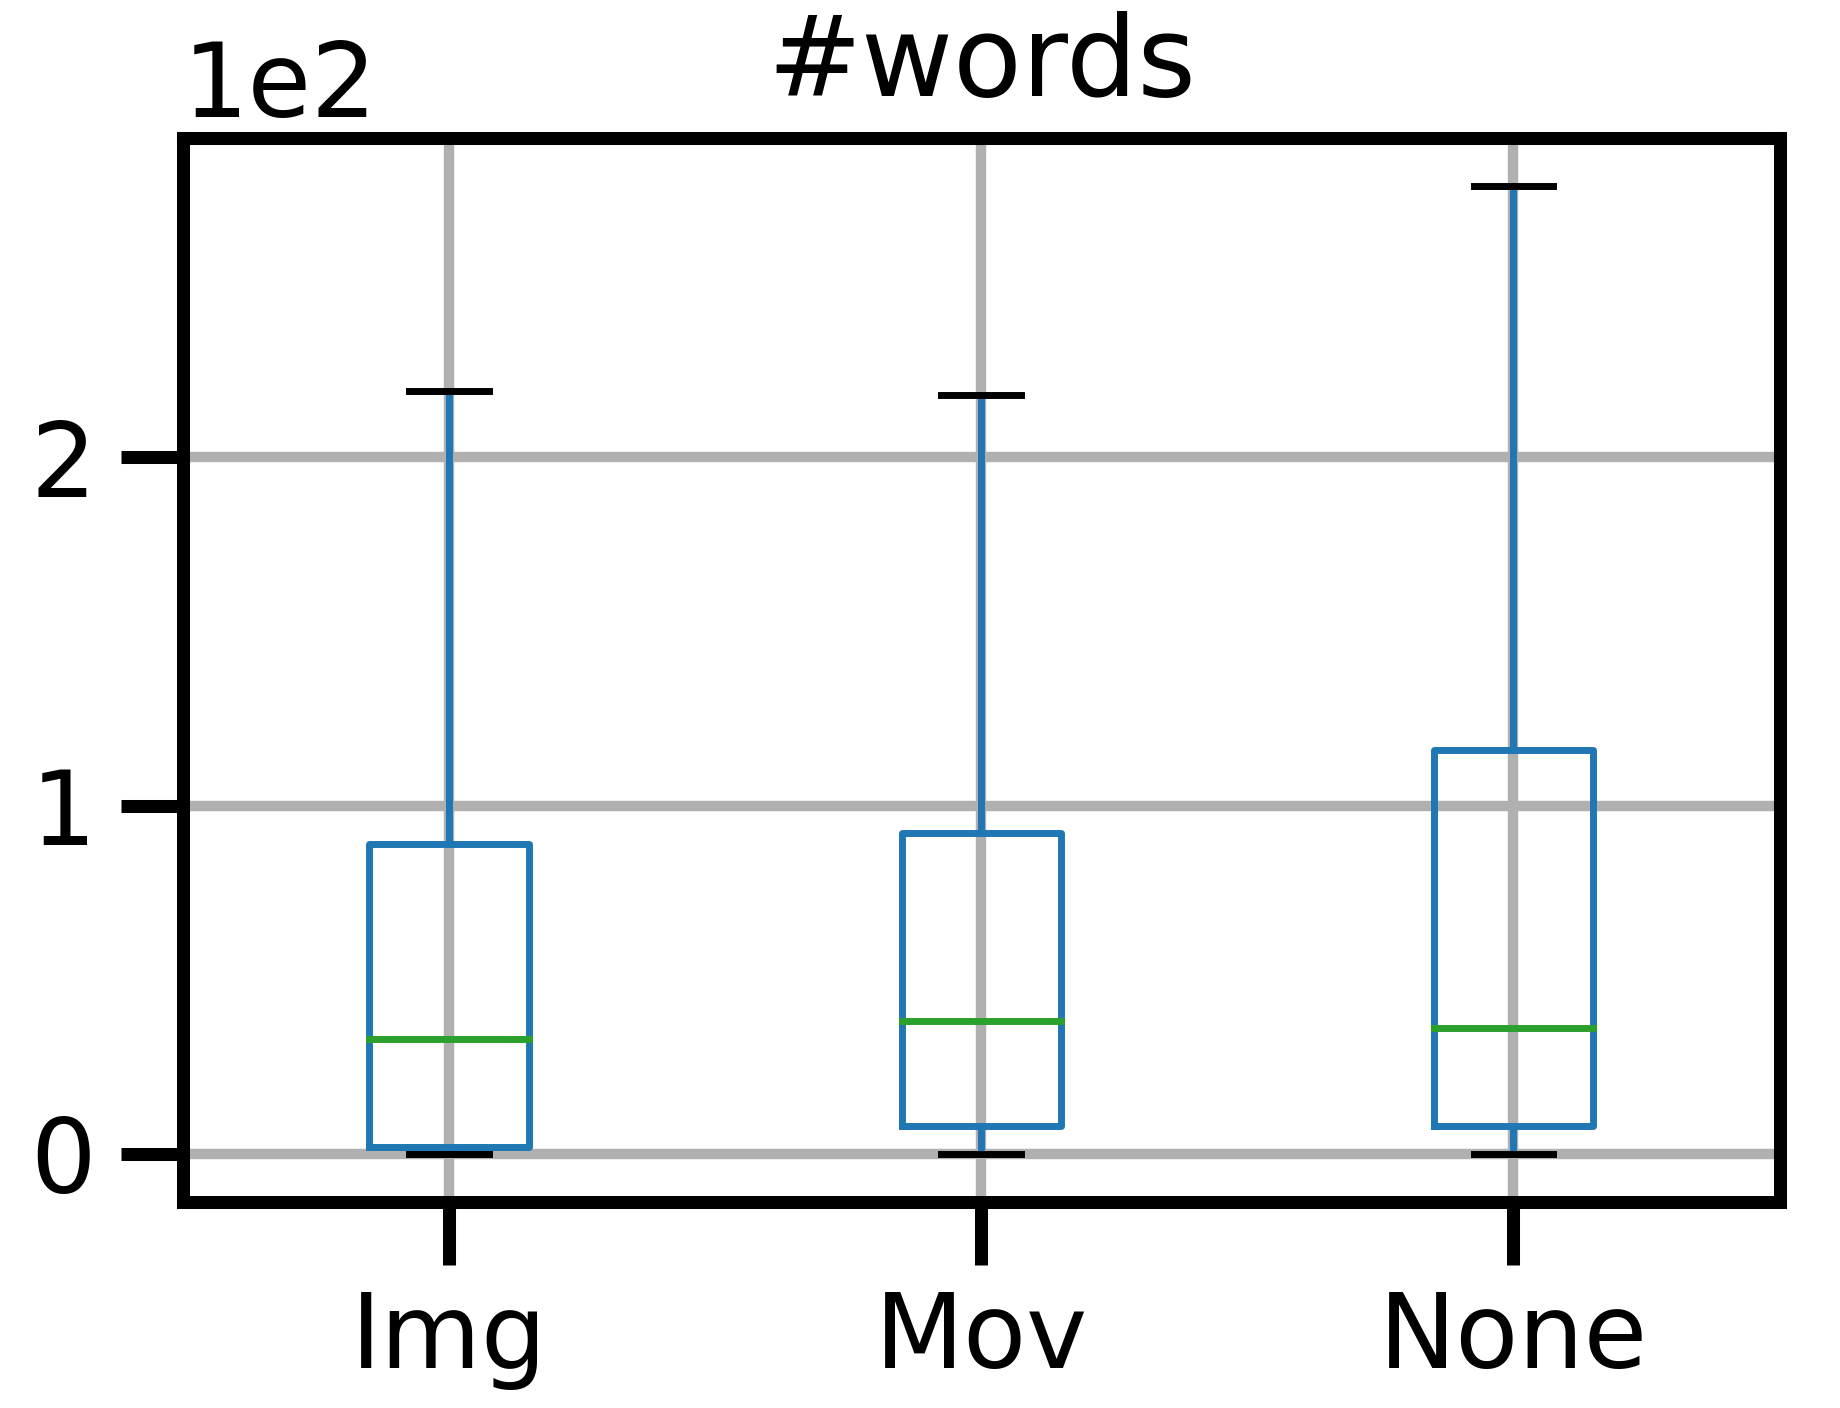
\includegraphics[width=0.5\linewidth]{tex-kondo/figures/words.png}
%     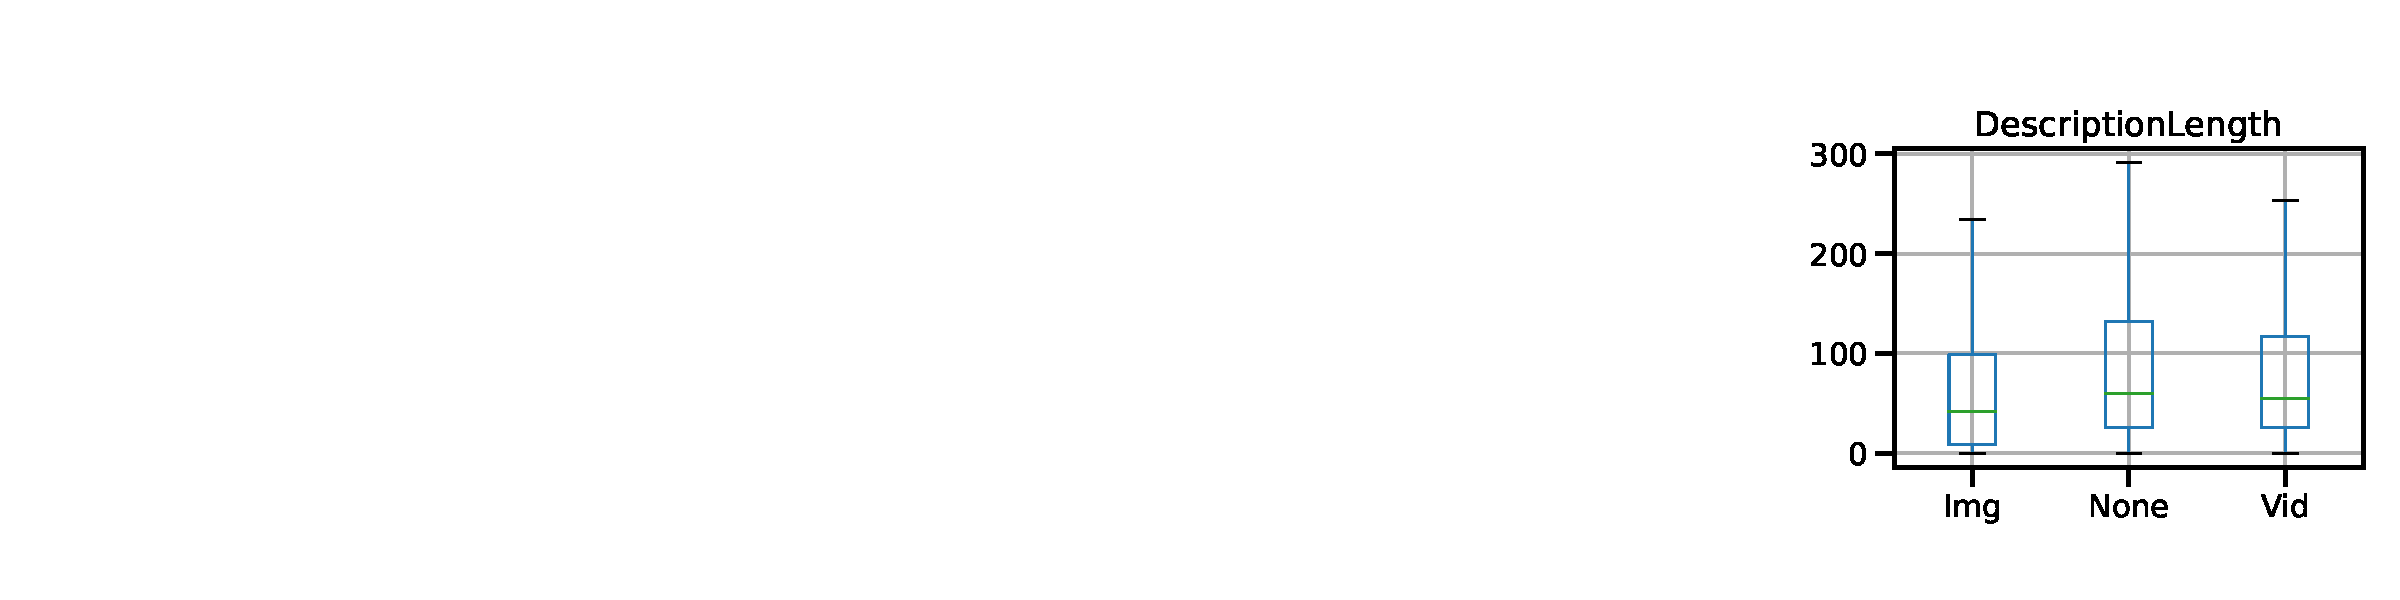
\includegraphics[width=0.5\linewidth]{./figures/words.pdf}
%     %\caption{Distributions of words written in issue reports. }
%     %\caption{Boxplots of \# of words written in the description }
%     % \caption{The attribute in the Report dimension}
%     \caption{Distribution of the number of words in the descriptions of issue reports (``Report'' dimension)}
%     \label{fig:words}
% \end{figure}
%\textbf{DescriptionLength of visual issue reports is 
%similar to the others.}

\fig{fig:words} shows the distributions in the number of words written in descriptions of issue reports. The median of DescriptionLength was 42.0 words in Img, 54.5 in Vid, and 60.0 in None. 
Compared with $Vid$ and $None$, the number of words in $Vid$ is slightly smaller than that of the non-visual ones. However, no statistically significant differences are observed between them (p $>$ 0.01). This implies that reporters write as many texts to describe the contents of videos as text-only reports. 

Shedding light on $Img$, the number of words in $Img$ is smaller (42 words) than 
that in $None$ (60 words) with a statistical significant difference (p $<$ 0.01). 
Compared with $Vid$, the median in $Img$ is smaller than that in $Vid$ (55 words). 
However, there is no statistically significant difference between $Img$ and $Vid$.%, p $>$ 0.01 
\vspace{-0.2cm}%これは本当は入れたくないがスペースがない
\summarybox
%{Answer to RQ1}
{
% {\bf RQ1: }{No, visual issue reports still require reporters 
% to write similar amounts of texts to describe bugs. 
{\bf RQ1: }{Issue reports with images are described in fewer words than non-visual issues, but still issue reports with videos require the same amount of words as non-visual issue reports. 
}}

\subsection*{RQ2: \RQtwo{}}
% \begin{figure}[t]
%     \centering
%     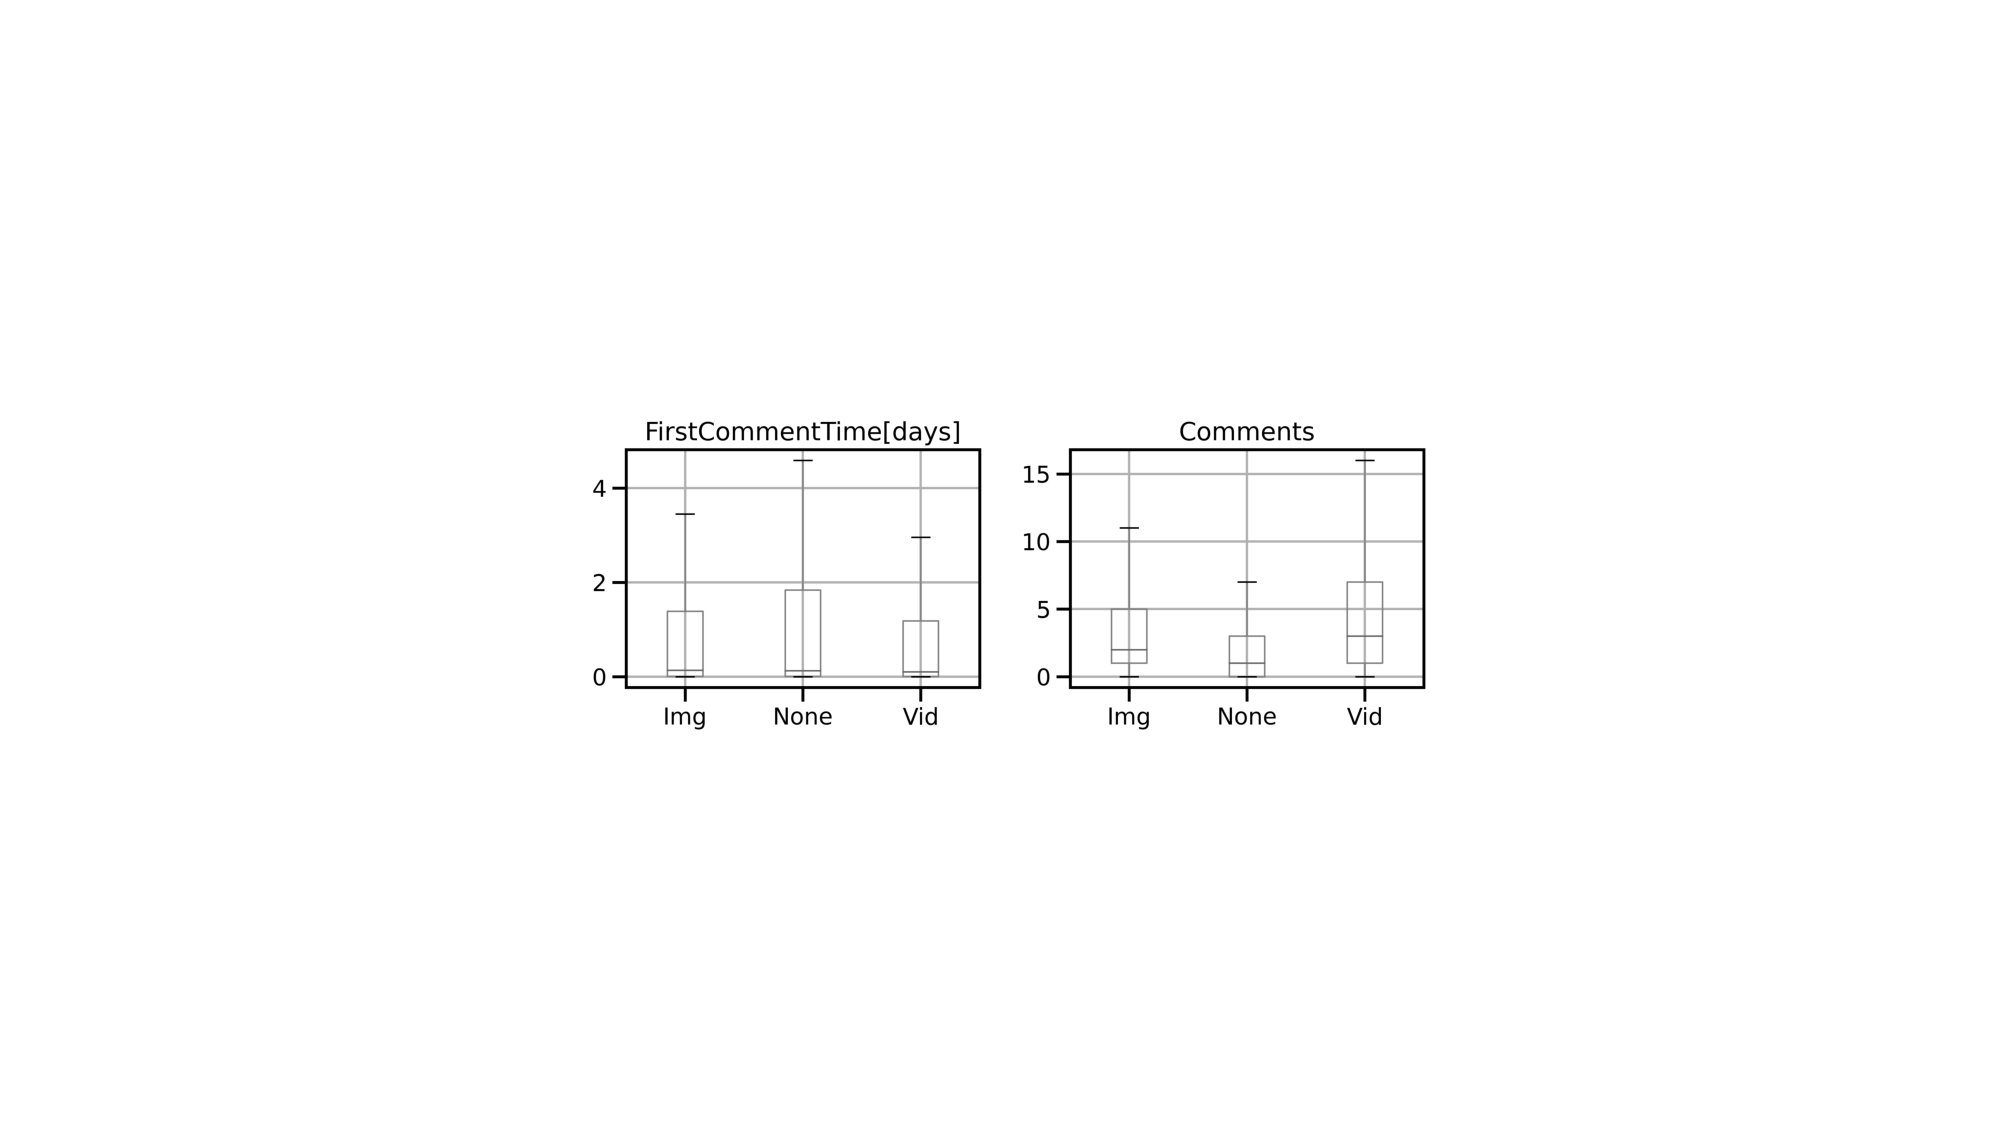
\includegraphics[width=1\linewidth]{./figures/discussions.pdf}
%     %\caption{Amount of texts written in issue reports. }
%     % \caption{The attributes in the Discussion dimension}
%     \caption{Distribution of days to receive the first comments and the number of comments (``Discussion'' dimension)}
%     \label{fig:discussion}
% \end{figure}


\fig{fig:discussion} shows the distributions of the number of comments and the days to receive the first comments. 
We observed that the interquatile range (i.e., the box) of $FirstCommentTime$ in the $Vid$ category are the largest, whereas that of the issue reports in the $Img$ category are the shortest. 
However, the median in the three categories are similar and no significant differences are observed ($Img$: 0.24 days, $Vid$: 0.40 days, $None$: 0.32). 

Also, in terms of $Comments$, the median and the interquatile range are almost same across the three categories, and no significant differences are observed. 
% Hence, the visual issue reports are not strongly related to active discussions.  
\vspace{-0.2cm}%これは本当は入れたくないがスペースがない
\summarybox
%{Summary of RQ2}
{{\bf RQ2: }{
    % Yes, visual issue reports are 3-times likely to receive more comments than reports without images or videos. 
    Visual issue reports do not lead to active discussions in terms of the number of words and the first response time. 
}}
\subsection*{RQ3: \RQthree{}}
\fig{fig:resolvedtime} shows the distribution of days between when the issue report was created and when the issue report was closed. The median of non-visual issues are larger (5.96 days) than that of $Img$ (4.78 days) and $Vid$ (5.70 days). Also, the interquatile range of $Img$ is smaller than the others. However, no statistically significant differences between any pairs are observed.  

\vspace{-0.2cm}%これは本当は入れたくないがスペースがない
\summarybox
%{Summary of RQ3}
{{\bf RQ3: }{
    % No, resolution time of visual issue reports is longer than that of other issue reports.
The median of resolution time in non-visual issue reports are larger than that in visual issue reports but no statistically significant difference are observed. 
}}




